\documentclass[10pt]{ujarticle}
 \usepackage[top=30truemm, bottom=30truemm, left=25truemm, right=25truemm]{geometry}
 \usepackage{ascmac}
 \usepackage{amssymb}
\usepackage{amsmath}
 \usepackage{bm}
 \usepackage[dvipdfmx]{graphicx,color}
 %\usepackage[dviout]{graphicx}
\begin{document}

\tableofcontents
\clearpage

\section{目的}
光には、波動性と粒子性の2重性がある。ある時は粒子のようにふるまい、ある時は波のようにふるまう。今回の実験では、日常概念での「粒子」や「波動」をそのまま当てはめることのできない光子の性質を確かめる。

\section{原理}

\subsection{光とは}
電子のエネルギー状態が、高エネルギー状態から低エネルギー状態へ変化した時、このエネルーの差分を原子の外に波動エネルギーとして放出する。この波動エネルギーを電磁波・光と呼ぶ。
位置$\bm{r}$、時間tにおける電磁波は以下の式で表される。
\begin{itemize}
\item 電場:$\bm{E} (\bm{r}, t) = \bm{E_0} \sin (\omega t - \bm{k} \cdot \bm{r} ) $
\item 磁場:$\bm{B} (\bm{r}, t) = \bm{B_0} \sin (\omega t - \bm{k} \cdot \bm{r} ) $
\end{itemize}
$\bm{E_0}, \bm{B_0}$:定数、 $\bm{k}$:波数ベクトル、 $\omega$:角振動数とする。

\subsection{光の干渉}
光の波動性を見る1つの実験として、干渉実験がある。以下、光の干渉の原理について述べる。
\subsubsection{線状光源}
直線に並んだ振幅、周波数が互いに等しいN個の光源を考える。各光源は等しい初期位相角をもっていると仮定する。ここで、j番目の光源が$r_j$離れた点で作る電場$E_j$は
\[
E_j = E_0 \sin(\omega t - k r_j)
\]
と書ける。今、$E_0 \varpropto 1/{r_j}$なので、定数$C_0$を用いて
\[
E_j = \frac{C_0}{r_j} sin(\omega t - k r_j)
\]



さらに、この光源を無限に並べた線状光源を考える。ここで、考えている状況は、各光源は非常に弱く、光源の数Nは極めて多く、光源間の間隔が無視できるほど小さい状況である。ここで、Dを線状光源全体の長さとすると、線状光源の微小部分$\delta y_i$個の光源を含んでいる。(ここで、光源はM個の微小部分に分けられているとする。$1 \leq i \leq M$)
\\
\begin{figure}[b]
\begin{center}
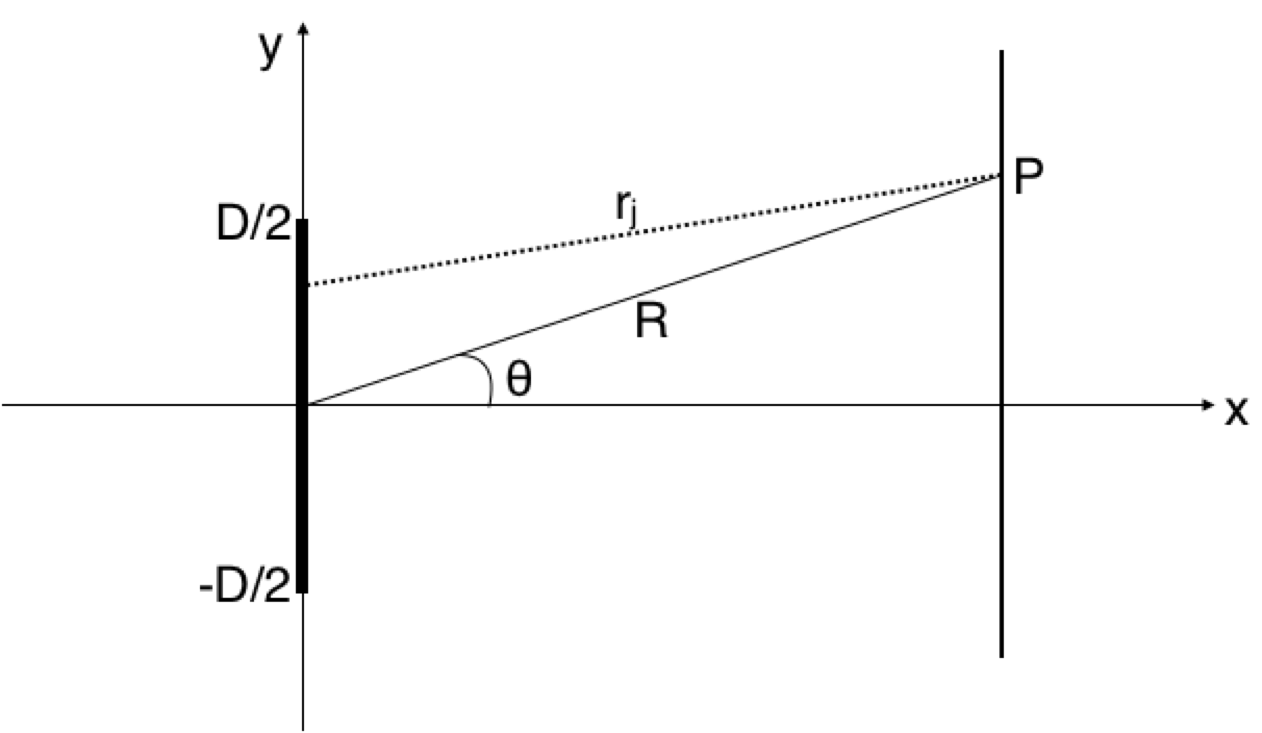
\includegraphics[width=6cm, bb = 0 0 600 200]{SummerChallenge_lineray.png}
\caption{線状光源}
\end{center}
\end{figure}

\clearpage
このとき$\delta y_i$がPに作る電場は、
\[
E_i = \frac{C_0}{r_i} \sin(\omega t- k r_i ) \frac{\delta y_i N}{D}
\]
となる。ただし、$\delta y_i$は微小であり、この微小範囲内の各光源からPまで距離は一定であるとする。さらに一定値の$C_L$を
\[
C_L = \frac{1}{D}  \lim_{N \to \infty} (C_0 N)
\]
と定義できる。M個の全部分によるPでの電場は、
\[
E = \sum_{i=1}^M \frac{C_L}{r_i} \sin(\omega t - k r_i) \delta y_i
\]
最後に、$\delta y_i$は無限小になるはずで、
\[
E = C_L \int_{-D/2}^{D/2} \frac{\sin(\omega t - k r)}{r} dy
\]
となる。ここで、$r = r(y)=\sqrt{R^2 \cos^2 \theta + (R\sin \theta - y )^2}$である。


\subsubsection{単スリット}
まず、単スリットの場合どのように干渉が起こるかを確かめる。振幅、周波数が互いに等しい長さDの線状光源を考える。線状光源の中心からyだけ離れた光源の微小部分dyが、中心からxy平面上の角$\theta$の方向にRだけ離れた点Pに作る電場は、
\[
dE = \epsilon \frac{\sin(\omega t - kr)}{r} dy
\]
$r(y)$を$y$でテイラー展開すると、
\begin{eqnarray*}
r &=&r(0) + \frac{\partial r(0)}{\partial y} y + \frac{1}{2!} \frac{\partial^2 r(0)}{\partial y^2} y^2 + \cdots \\
&=&R - y\sin\theta + \frac{y^2}{2R} \cos^2 \theta
\end{eqnarray*}
となる。いま、$R \gg y$なので、第3項以降は無視できる。
\[
dE = C_0 \frac{sin(\omega t -k(R- ysin\theta ))}{R- ysin\theta} dy
\]
これの分母は$R \gg y$より$R$としてよいので、
\[
dE = C_0 \frac{sin(\omega t -k(R- ysin\theta ))}{R} dy
\]
これは、Rが十分大きいとき、$\theta$の全ての値に対して正しい。
\begin{eqnarray*}
E &=& C_L \int_{-D/2}^{D/2} \frac{\sin(\omega t - k( R - y\sin\theta ))}{R} dy \\
%&=& \frac{C_L}{R} \int_{-D/2}^{D/2} sin(\omega t - k( R - ysin\theta )) \\
&=& \frac{C_L}{R(kD/2)\sin\theta} \sin(\frac{kD}{2} sin\theta) sin(\omega t -kR) \\
&=& \frac{C_L D}{R\beta} sin\beta \sin(\omega t - kR)
\end{eqnarray*}
$\beta = \frac{kD}{2} \sin\theta$とすると、以上のようになり、線状光源が作る電場が導かれた。このとき、強度は$I(\theta) = <E^2>_T$で求められるので、
\begin{eqnarray*}
I(\theta) &=& < E^2>_T\\
&=& <sin^2(\omega t - kR)>_T (\frac{C_L D}{E})^2 (\frac{sin\beta}{\beta})^2
\end{eqnarray*}
$<E^2>_T$は$E^2$の十分に長い時間発展で、周期 $2\pi / \omega$とすると、
\begin{eqnarray*}
 <sin^2(\omega t - kR)>_T  &=& \frac{\omega}{2\pi} \int_{0}^{2\pi / \omega} \sin^2(\omega t - kR) dt \\
 %&=& \frac{\omega}{2\pi} \int_{0}^{2\pi / \omega} \frac{1}{2} (1-cos(2(\omega t -kR))) dt \\
 &=& \frac{1}{2} 
 \end{eqnarray*}
 より、
\[
I(\theta) = \frac{1}{2} (\frac{C_L D}{R})^2 (\frac{sin \beta}{\beta})^2
\]
$I(0)$を求めると
\[
I(0) = \frac{1}{2} (\frac{C_L D}{R})^2
\]
なので、
\[
I(\theta) = I(\theta) (\frac{\sin \beta}{\beta})^2
\]
と求まる。光の強度の変化と観測位置の関係は以下のように表される。\\

\begin{figure}[h]
\begin{center}
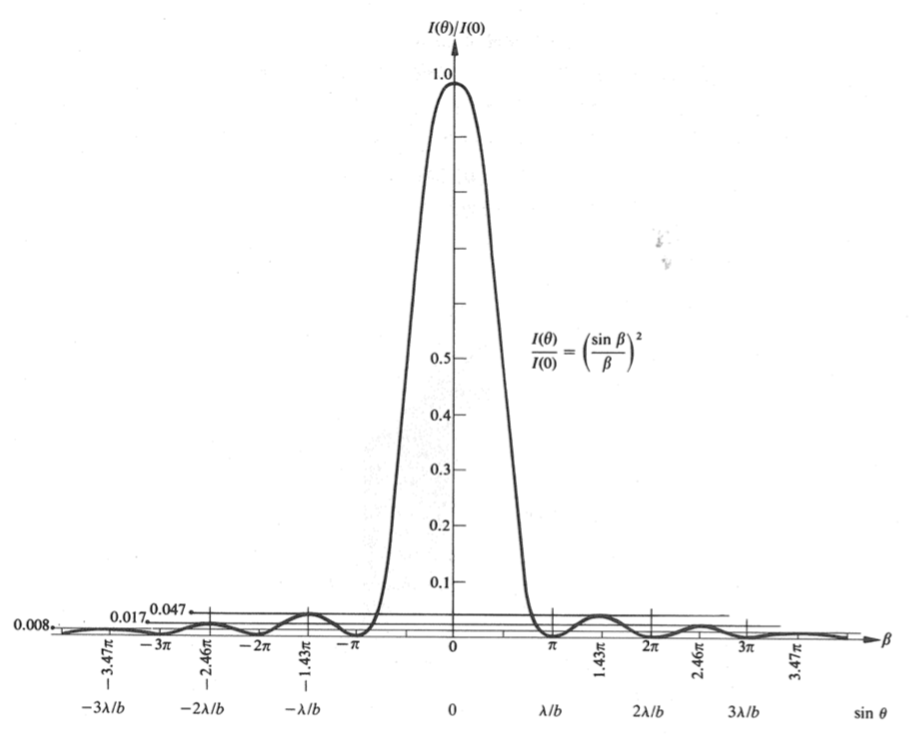
\includegraphics[width=10cm, bb = 0 0 1000 800]{SummerChallenge_slit.png}
\caption{単スリットでの光の強度と角度の関係}
\end{center}
\end{figure}

\clearpage

\subsubsection{2重スリット}
図のような、幅$b$、中心間隔$a$の2本の長いスリットがあるとする。スクリーン上のある点の光波に対する式を得るには、2つの電場の和になるので、
\begin{eqnarray*}
E &=& \frac{C_L}{R} \int_{-b/2}^{b/2} F(z) dz + \frac{C_L}{R'} \int_{a-b/2}^{a+b/2} F(z) dz \\
&\simeq& \frac{C_L}{R} \int_{-b/2}^{b/2} F(z) dz + \frac{C_L}{R} \int_{a-b/2}^{a+b/2} F(z) dz \\ 
\end{eqnarray*}
ここで、
\begin{eqnarray*}
F(z) &=& sin(\omega t - k(R-zsin\theta)) \\
\alpha &=& \frac{ka}{2} \sin\theta \\
\beta &=& \frac{kb}{2} \sin\theta
\end{eqnarray*}
これより、この式を簡単にすると、
\[
E = 2 \frac{C_L b}{R} \frac{\sin\beta}{\beta} \cos\alpha \sin(\omega t -kR + \alpha)
\]
であり、単スリットの時と同様に強度$I(\theta) = <E^2>_T$を求めると、$I(\theta) = \frac{1}{2} (\frac{C_L b}{R})^2$より
\[
I(\theta) = 4I_0 (\frac{\sin \beta}{\beta})^2 \cos^2 \alpha
\]
となる。\\
\\
\\
\\
\begin{figure}[h]
\begin{center}
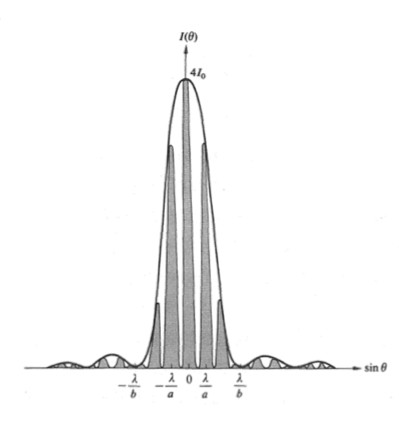
\includegraphics[width=8cm, bb = 0 0 400 300]{SummerChallenge_2slits.png}
\caption{2重スリットでの光の強度と角度の関係}
\end{center}
\end{figure}

\subsubsection{参考文献}
\begin{itemize}
\item 「フーリエ光学(第3版)」森北博巳(森北出版株式会社)2012年初版
\end{itemize}
\clearpage


\subsection{光子を数える}
光量が極端に少なくなると、光は光子として離散的になり、その数を数えることができるようになる。「光子数を数える」ということで、光の粒子性を観測することができる。どのような機器で測定するかは、次章にて述べる。


\section{実験装置}
\subsection{実験のセットアップ}
\subsection{信号発生器、NIMモジュール、MPPC、EASIROC、可動ステージ等の説明}
\subsection{データ収集の方法}

\section{データ解析}
\subsection{MPPCで取得されるデータの解析}
\subsection{Poisson統計}
\subsection{干渉縞の再現}

\section{まとめ}

\end{document}
